\documentclass{article} % For LaTeX2e
\usepackage[final]{colm2025_conference}
\usepackage{graphicx}
\usepackage{amsmath}
\usepackage{microtype}
\usepackage{hyperref}
\usepackage{url}
\usepackage{booktabs}
\usepackage{lineno}
\usepackage{amsmath}
\usepackage{algpseudocode}
\usepackage{algorithm}
\usepackage{graphicx} % Required for inserting images
\usepackage{subcaption} % For subfigure arrangement
\usepackage{caption}

\definecolor{darkblue}{rgb}{0, 0, 0.5}
\hypersetup{colorlinks=true, citecolor=darkblue, linkcolor=darkblue, urlcolor=darkblue}

\usepackage{etoolbox}
\makeatletter
\patchcmd{\@maketitle}
  {Published as a conference paper at COLM 2025}
  {}
  {}
  {}
\makeatother
\title{Week 5 Report}

% Authors must not appear in the submitted version. They should be hidden
% as long as the \colmfinalcopy macro remains commented out below.
% Non-anonymous submissions will be rejected without review.

\author{Mu Junrong}

% The \author macro works with any number of authors. There are two commands
% used to separate the names and addresses of multiple authors: \And and \AND.
%
% Using \And between authors leaves it to \LaTeX{} to determine where to break
% the lines. Using \AND forces a linebreak at that point. So, if \LaTeX{}
% puts 3 of 4 authors names on the first line, and the last on the second
% line, try using \AND instead of \And before the third author name.

\newcommand{\fix}{\marginpar{FIX}}
\newcommand{\new}{\marginpar{NEW}}

\begin{document}

\ifcolmsubmission
\linenumbers
\fi

\maketitle

\begin{abstract}
This report focuses on the introduction to transformers and Large Language Models (LLMs). Fundamental concepts including transformer architecture, self-attention and Feed-Forward network (FFN) are explained. The report also examines the training and post-training processes of Large Language Models (LLMs), such as GPT.
\end{abstract}

\section{Transformer Architecture}
The Transformer architecture is a deep learning model architecture introduced in the 2017 paper "Attention is All You Need" by Vaswani et al (\cite{vaswani2017attention}). It's especially well-known because it's the foundation of modern large language models (LLMs) including Bidirectional Encoder Representations from Transformers (BERT) and generative pre-train transformers (GPT). The Transformer architecture has two stacks, encoder stack and decoder stack respectively. 

The Transformer uses self-attention to process sequences, allowing the model to capture relationships between tokens simultaneously, instead of step-by-step evaluation by Recurrent Neural Network (RNNs).
\begin{figure} [H]
    \centering
    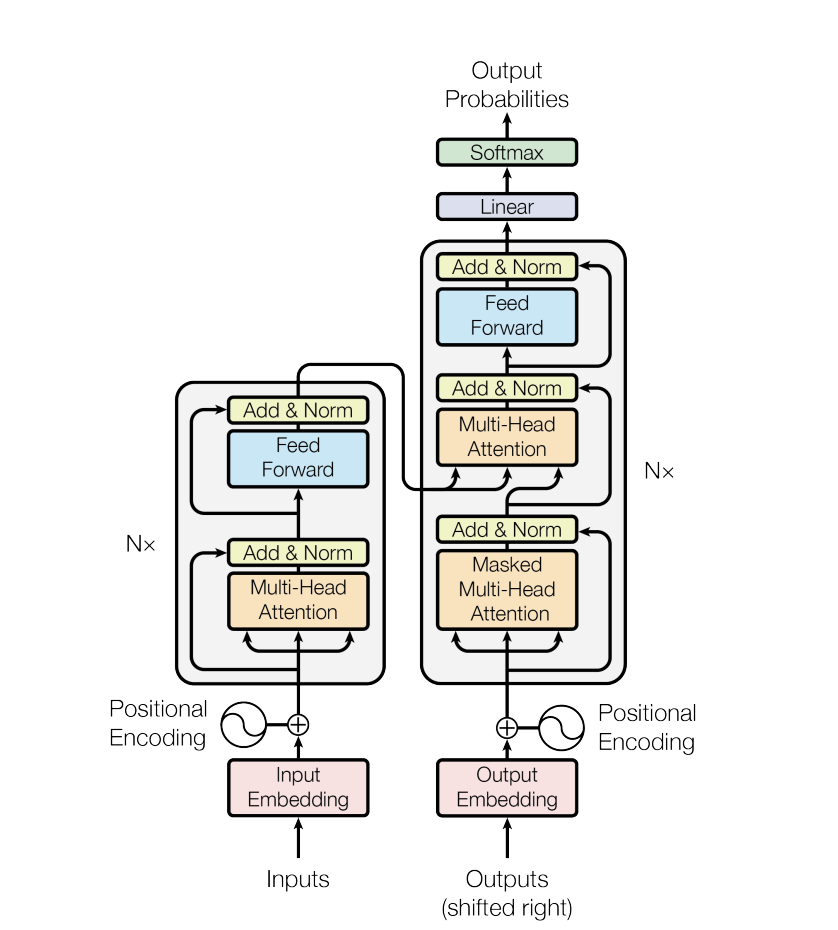
\includegraphics[width=0.5\linewidth]{Transformer_Architecture.png}
    \caption{The Transformer  model architecture introduced in the paper "Attention is All You Need".}
    \label{fig:enter-label}
\end{figure}

\subsection{Encoder stack}
The encoder stack in the Transformer architecture is used for understanding and representing the input. It transforms raw input tokens into rich, contextual embeddings that capture meaning and relationships between tokens. 
Any input is split into tokens. Each token is converted into a fixed-size vector using an embedding matrix, and positional encoding is added to each word vector. This processed input is passed to a stack of N identical encoder layers, which consist of Multi-head attention and a Feed-Forward Network (FFN). 

\subsubsection{Single-head attention and Multi-head attention}
Self-attention (\cite{liu2021multihead_vs_single}) helps a model understand how each word in a sentence relates to the others, by assigning attention scores. These scores decide how much focus each word should give to the rest.
Each token is turned into three vectors, Query (Q), Key (K) and Value (V), by $
Q = XW^Q, K=XW^K, V=XV^V
$, where \( W^Q, W^K, W^V \in \mathbb{R}^{d_{\text{model}} \times d_k} \) are trainable weight matrices.

The single-head scaled attention score between token i and token j is the dot product of their Q and K vectors, since dot product represents the similarity between two vectors. The attention score is scaled by $\sqrt{d_k}$ to prevents large dot products (for stable gradients).
\[
\text{Attention score}_{i,j} = \frac{Q_i \cdot K_j^T}{\sqrt{d_k}}
\]

The attention matrix is given by:
\[
\text{Attention}(Q, K, V) = \text{softmax} \left( \frac{QK^T}{\sqrt{d_k}} \right) V
\]
Where $QK^T$ computes the similarity scores between each token pair, and $\text{softmax}$ turns scores into probabilities (attention weights). By doing so, a matrix of the same shape as the input is computed, which represents new context-aware vectors for each token.

In multi-head self-attention, instead of using a single set of $Q, K, V$ projections, multiple sets (heads) are used, each head pays attention to different aspects of the input. Each head is given by
 \[
\text{head}_i = \text{Attention}(XW_i^Q, XW_i^K, XW_i^V)
    \]
    
for each \( i \in \{1, \dots, h\} \)
    
All heads are then concatenated and applied to compute the final linear transformation
   
    \[
    \text{MultiHead}(Q, K, V) = \text{Concat}(\text{head}_1, \dots, \text{head}_h)W^O
    \]


Where:
\( W^O \in \mathbb{R}^{hd_v \times d_{\text{model}}} \) is a learnable projection matrix. 

\subsubsection{Add and Norm layer}
The Add and Norm layer helps with stability, training speed, and gradient flow by applying Residual connection (Add) and Layer normalization (Norm).

The Residual connection (Add) enables grdient flow and allows the model to preserve information from the earlier layers. The formula is given by
\[z=x + Sublayer(x)\]
where \( x \in \mathbb{R}^{d_{\text{model}}} \), and $Sublayer(x)$ is the output of attention or feedforward.

The Layer normalization (Norm) improves training stability and helps the model converge faster by normalizing each vector. The normalized vector is given by
\[
LayerNorm(x) = \gamma\frac{x_j - \mu_j}{\sqrt{\sigma_j^2 + \epsilon}} + \beta
\]
where $\gamma$ and $\beta$ are learnable parameters. (\cite{chafiqui2024deepdive_transformer})

\subsubsection{Feed-Forward Network (FFN)}
The FeedForward Network (FFN) in a Transformer processes each token vector independently after self-attention (\cite{zhang2024transformer_explain}). It adds non-linearity and transformation capacity to the model. The final output of each iteration is given by 
\[Output = LayerNorm(x+FFN(x))\]

Let \( x \in \mathbb{R}^{d_{\text{model}}} \) be the input token vector at some position. The FFN is given by
\[
\text{FFN}(x) = W_2 \cdot \text{ReLU}(W_1 \cdot x + b_1) + b_2
\]
\( W_1 \in \mathbb{R}^{d_{\text{ff}} \times d_{\text{model}}} \), \( W_2 \in \mathbb{R}^{d_{\text{model}} \times d_{\text{ff}}} \), \( b_1 \in \mathbb{R}^{d_{\text{ff}}}, b_2 \in \mathbb{R}^{d_{\text{model}}} \), \( d_{\text{model}} \) is the hidden size, and the ReLU function is defined as:
\[
\text{ReLU}(x) = \max(0, x) = 
\begin{cases} 
x & \text{if } x \geq 0 \\
0 & \text{if } x < 0 
\end{cases}
\]
   
\subsection{Decoder stack}
The decoder stack in the Transformer architecture is used for generating output sequences—one token at a time—based on both prior outputs and the encoder’s context. It’s used for machine translation and text generation, summarization. The decoder stack consists of N layers and has similar procedure as the encoder, but with an extra attention layer to attend to the encoder’s output.

In the decoder stack, any output is split into tokens and converted into a vector using an embedding matrix, and positional encoding is added. The processed output vectors are passed to a masked multi-head attention and the add and Layer Norm. Next, Encoder-Decoder (cross) attention is applied, and finally the Feed-Forward Network (FFN).

\subsubsection{Masked multi-head attention}
In decoder self-attention, the future token is unwanted. Thus, a causal mask is introduced. A mask matrix \( M \) is added to prevent looking ahead where M is defined as
\[
M_{i,j} = 
\begin{cases} 
0 & \text{if } j \leq i \\ 
-\infty & \text{if } j > i 
\end{cases}
\]

The masked attention score is given by
\[
\text{Masked attention score} = \frac{QK^\top}{\sqrt{d_k}} + M
\]
The attention matrix is given by
\[ Attention (Q, K, V) = \text{softmax}(\frac{QK^\top}{\sqrt{d_k}} + M) V \] \quad where each row sums to 1, future positions = 0\\
The masked multi-head attention is given by \[
    \text{MultiHead}(Q, K, V) = \text{Concat}(\text{head}_1, \dots, \text{head}_h)W^O
    \] where
    \[
\text{head}_i = \text{Attention}(XW_i^Q, XW_i^K, XW_i^V)
    \]

\subsubsection{Encoder-Decoder (cross) attention}
The encoder-decoder attention allows the decoder to access and focus on relevant parts of the input sequence (i.e., the encoder’s output). It also learns alignment between input and output tokens.

Q, K, V are computed respectively by
\[ Q = X_{\text{dec}} W^Q\]
\[K = H_{\text{enc}} W^K \]
\[ V = H_{\text{enc}} W^V \]
where \( X_{\text{dec}} \in \mathbb{R}^{T_{\text{dec}} \times d_{\text{model}}} \) is the decoder's input so far (masked self-attention output), and \( H_{\text{enc}} \in \mathbb{R}^{T_{\text{enc}} \times d_{\text{model}}} \) is the encoder output (which is fixed in full sequence).

Then using the standard multi-head attention, multi-head attention is computed by
\[
\text{MultiHead}(Q, K, V) = \text{Concat}(\text{head}_1, \dots, \text{head}_h)W^O
    \] where
    \[
\text{head}_i = \text{Attention}(XW_i^Q, XW_i^K, XW_i^V)
    \]


\section{Training process of Large Language Model (LLM)}
LLM training involves teaching the model to predict the next token in a sequence of text, given all previous tokens. There are mainly two types of LLm, namely generative pre-train transformers (GPTs) and Bidirectional Encoder Representations from Transformers (BERT).

The aim of LLM training is to minimize prediction error (loss) on text data.

\subsection{GPTs v.s. BERTs}
Generative pre-train transformers (GPTs) aims to lean to auto-regressively generate text. It uses the decoder-stack only architecture, where self-attention is masked, allowing only left-to-right attention. It is widely used in ChatGPT and its invariants (\cite{radford2018improving}).

For example, in the sentence "the cat sat on the mat", the word "sat" is generated by paying attention to all the words in front (i.e., "the" and "cat").

On the other hand, Bidirectional Encoder Representations from Transformers (BERT) uses the encoder-stack only, where each token attends to all other tokens, bidirectionally. The Masked Language Modeling (MLM)is used, which randomly masks some tokens in the input, and the model leanrs to fill in the blanks using both left and right context (\cite{devlin2018bert}).

For example, in the sentence "the cat sat on the mat", the word "sat" is generated by paying attention to all the other words (i.e., "the", "cat" and "on the mat").

\subsection{Pre-training process}
Before training LLMs, training goal needs to be decided (i.e., whether causal learning model is used for GPTs, or masked learning model is used for BERT). Raw data is then collected and cleaned. The raw data are converted to tokens using a tokenizer (e.g., Byte-Pair Encoding (BPE)), to separate the war data into smaller pieces. 

Next, the training model is initialized. The size of layers $N$, the hidden size, the number of attention heads and the initial weights are initialized. 

\subsection{Training process: forward passing}
During training, Each token ID is mapped to a dense vector
    \[
    x_i = \text{Embedding}(t_i) + \text{PositionalEncoding}(i)
    \]
where $x \in \mathbb{R}^{T \times d_{\text{model}}}$ and where $T$ is the sequence length. The vectors are then passed to the transformer, and the final output h is given by
\[h=Transformer(x)\]
where \(h \in \mathbb{R}^{T \times d_{\text{model}}} \).

Secondly, to predict the next token, a linear layer is used on each \(h_t\) and the logit for position token $t$ is given by
\[
z_t = W \cdot h_t + b
\]
where $h_t$ is the hidden representation for each position token $t$, \( W \in \mathbb{R}^{|V| \times d_{\text{model}}} \) (i.e., a matrix that transforms from hidden space to output space).

Thirdly, softmax function is then applied to logits, to convert logits into probabilities
\[
p_i = \frac{e^{z_i}}{\sum\limits_{j=1}^{|V|} e^{z_j}}
\]
where $p$ is a probability distribution ($p \in \mathbb{R}^{|V|}$).

Next, loss is computed and minimized (i.e., the goal of training is to predict token correctly). For a position, a predicted probability vector $p$, and the true token being class $k$, the loss is
\[
\mathcal{L}_t = -\log(p_k)
\]
Using the one-hot notation, the loss is given by
\[
\mathcal{L}_t = -\sum_{i=1}^{|V|} y_i \log(p_i)
\]

Where \( p_i \) is the softmax probability for class \( i \), and \( y \) is the one-hot encoded true label such that
\[
    y_i = \begin{cases}
    1 & \text{if } i = k  \\
    0 & \text{otherwise}
    \end{cases}
    \]

Lastly, to update the parameters, backpropagation is done. Gradients of loss is computed with respect to all model weights, and flow back through transformer layers. The Adam or AdamW algorithm (\cite{loshchilov2017decoupled}) is used to update weights
\[
    \theta \leftarrow \theta - \eta \cdot \nabla_\theta L
    \]
\[
    {\theta} \leftarrow {\theta} - \eta_t \cdot {m}_t / (\sqrt{{v}_t} + \epsilon)
    \]


\section{Post training process of LLMs}
After an LLM (such as GPTs or BERTs) has been pre-trained, it often goes through one or more post-training stages to align it better with specific goals, tasks, or human preferences. 

\subsection{Supervised fine-tuning (SFT)}
Supervised fine-tuning is done to train the pre-trained model on labeled datasets (e.g. instruction–response pairs), with supervised learning (SL). The cross-entropy is computed, and parameters are updated using AdamW algorithm (in section 2.3)

\subsection{Reinforcement Learning from Human Feedback (RLHF)}
RLHF is a post-fine-tuning alignment method. It guides the model to generate outputs that align with human values or preferences, instead of following data patterns.

Firstly, the model is trained on a dataset of good prompts and responses, which provides a strong initial policy $\pi_\theta$. 

Next, annotators (i.e., human) compare several model outputs $y_1, y_2, \ldots$ for the same input $x$, ranking which they prefer. A reward function $R_{\phi}(x, y)$ is trained to model human preferences. The loss function is given by 
\[
\mathcal{L}_{\text{RM}} = -\log\sigma(R_{\phi}(x, y_{\text{better}}) - R_{\phi}(x, y_{\text{worse}}))
\]

Lastly, the language model is considered as a policy $\pi_\theta(y|x)$ and use Proximal Policy Optimization (PPO) to update it, maximizing human-aligned rewards.The objective function is defined as 
\[
\max_{\theta} \mathbb{E}_{x \sim D, y \sim \pi_\theta}[R_\phi(x, y) - \text{KL}(\pi_\theta||\pi_{\theta_0})]
\]


\bibliography{colm2025_conference}
\bibliographystyle{colm2025_conference}


\end{document}
